\renewcommand*\chappic{diff-crypt.pdf_tex}
\chapter{Differential cryptanalysis}
\label{ch:diff-crypt}
%
\section{MD4}
\label{ch:md4}
%
MD4 is a cryptographic hash function originally described in RFC~1186~\cite{rfc1186},
updated in RFC~1320~\cite{rfc1320} and obsoleted by RFC~6150~\cite{rfc6150}. It was
invented by Ronald Rivest in 1990 with properties given in Table~\ref{tab:md4}.
Since 1995~\cite{Dobbertin1998} successful attacks have been found to break collisions,
preimage and second-preimage resistance in MD4; including but not limited to~\cite{md4-2007} and
\cite{cryptoeprint:2005:151}. A Python~3 implementation derived from a previous Python version
is available at github~\cite{md4-py3k}.

\begin{table}[h]
  \begin{center}
    \begin{tabular}{lcl}
      block size           & 512 bits       & namely variable \texttt{block} in RFC~1320~\cite{rfc1320} \\
      digest size          & 128 bits       & as per section~3.5 in RFC~1320~\cite{rfc1320} \\
      internal state size  & 128 bits       & namely variables $A$, $B$, $C$ and $D$ \\
      word size            & 32 bits        & as per section~2 in RFC~1320~\cite{rfc1320} \\
    \end{tabular}
    \caption{MD4 hash algorithm properties}
    \label{tab:md4}
  \end{center}
\end{table}

A short summary of MD4's design is given:
Once padding and length extension has been applied, the message is split into 512-bit blocks
(i.e. 16 32-bit words). Four state variables $A$, $B$, $C$ and $D$ are initialized
with hexadecimal values:
\[
  \mathbf{[A]}\; \mathtt{01234567} \quad
  \mathbf{[B]}\; \mathtt{89abcdef} \quad
  \mathbf{[C]}\; \mathtt{fedcba98} \quad
  \mathbf{[D]}\; \mathtt{76543210}
\]
To process one block, three auxiliary functions are defined:
\begin{align}
  F(X,Y,Z) &= (X \land Y) \lor (\neg X \land Z) \\
  G(X,Y,Z) &= (X \land Y) \lor (X \land Z) \lor (Y \land Z) \\
  H(X,Y,Z) &= X \oplus Y \oplus Z
\end{align}

\begin{figure}[t]
  \begin{center}
    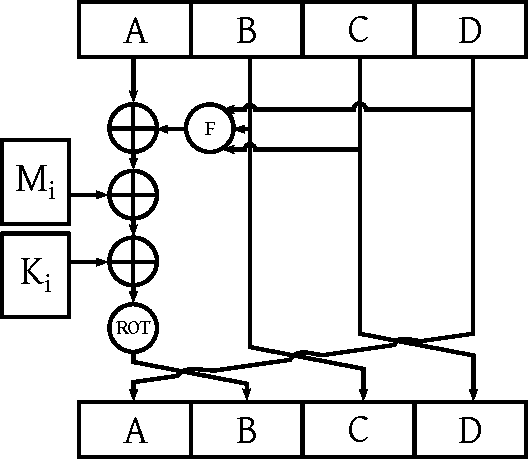
\includegraphics{img/md4.pdf}
    \caption{MD4 round function}
    \label{fig:md4-round-function}
  \end{center}
\end{figure}

\section{Differential notation}
\section{Addition example}
\section{Differential path}
